\chapter{回溯法}

\section{算法思想} %%%%%%%%%%%%%%%%%%%%%%%%%%%%%%

当把问题分成若干步骤并递归求解时,如果当前步骤没有合法选择,则函数将返回上一级递归调用,
这种现象称为回溯(backtrack)。正是因为这个原因,枚举递归算法常被称为回溯法。

回溯法 = 深搜 + 剪枝。树的深搜或图的深搜都可以。深搜一般用递归来写,这样比较简洁。

回溯法比暴力枚举法快的原因,在于:暴力枚举法,是每生成一个完整的解答后,
再来判断这个解答是否合法,而回溯法则在生成每一步中都进行判断,
而不是等一个答案生成完毕后再来判断,这样,在每一步进行剪枝,减少了大量的废答案。

\section{八皇后问题} %%%%%%%%%%%%%%%%%%%%%%%%%%%%%%

在8×8的棋盘上,放置8个皇后,使得她们互不攻击,每个皇后的攻击范围是
同行、同列和同对角线,要求找出所有解。如图~\ref{fig:eightQueens}所示。

\begin{center}
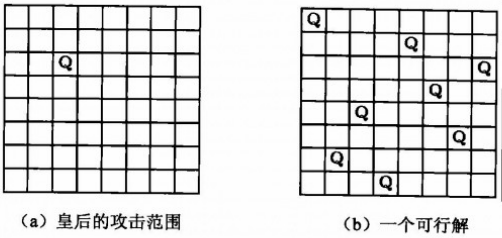
\includegraphics[width=240pt]{eight-queen.png} \\
\figcaption{八皇后问题}\label{fig:eightQueens}
\end{center}

\subsubsection{分析}
最简单的暴力枚举方法是,从64个格子中选一个子集,使得子集含有8个格子,且任意两个格子
都不在同一行、同一列或同一个对角线上。这正是子集枚举问题,然而64个格子的子集有$2^64$个,
太大了,这并不是一个很好的模型。

第二个思路是,从64个格子中选8个格子,这是组合生成问题。根据组合数学,有 $C_{64}^{8} \approx 4.426 \times 10^9$ 种方案,
比第一种方案优秀,但仍然不够好。

经过思考不难发现,由于每一行只能放一个皇后,那么第一行有8种选择,第二行有7中选择,…,
第8行有1中选择,总共有$8!=40320$个方案。如果用C[x]表示第x行皇后的列编号,则问题变成了一个
全排列生成问题,枚举量不会超过8!。

\subsubsection{代码}
\begin{Codex}[label=eight_queen.c]
#include <stdio.h>
#include <stdlib.h>

#define QUEENS 8 // 皇后的个数,也是棋盘的长和宽

static int total = 0;	// 可行解的总数
static int C[QUEENS] = {0};	// C[i]表示第i行皇后所在的列编号

/** 
 * @brief 输出所有可行的棋局,按行打印.
 * @return 无
 */
void output1() {
    int i, j;
    printf("No. %d\n", total);
    for (i = 0; i < QUEENS; ++i) {
        for (j = 0; j < QUEENS; ++j) {
            if (j != C[i]) {
                printf("0 ");
            } else {
                printf("1 ");
            }
        }
        printf("\n");
    }
}

/** 
 * @brief 输出所有可行的棋局,按列打印.
 *
 * http://poj.grids.cn/practice/2698/ , 这题需要按列打印
 *
 * @return 无
 */
void output() {
    int i, j;
    printf("No. %d\n", total);
    for (i = 0; i < QUEENS; ++i) {
        for (j = 0; j < QUEENS; ++j) {
            if (i != C[j]) {
                printf("0 ");
            } else {
                printf("1 ");
            }
        }
        printf("\n");
    }
}

/** 
 * @brief 检查当前位置(current, column)能否放置皇后.
 *
 * @param[in] current 当前行
 * @return 能则返回1,不能则返回0
 */
static int check(const int current, const int column) {
    int ok = 1;
    int j;
    for(j = 0; j < current; ++j) {
        // 两个点的坐标为(current, column), (j, C[j])
        // 检查是否在同一列,或对角线上
        if(column == C[j] || current - j == column - C[j] || 
            current - j == C[j] - column) {
            ok = 0;
            break;
        }
    }
    return ok;
}

/** 
 * @brief 八皇后,回溯法
 *
 * @param[in] current 搜索当前行,该再哪一列上放一个皇后
 * @return 无
 */
static void search(const int current) {
    if(current == QUEENS) {  // 递归边界,只要走到了这里,意味着找到了一个可行解
        ++total;
        output();
    } else {
        int i;
        for(i = 0; i < QUEENS; ++i) {  // 一列一列的试
            const int ok = check(current, i);
            if(ok) {  // 如果合法,继续递归
                C[current] = i;
                search(current + 1);
            }
        }
    }
}

// 表示已经放置的皇后
// 占据了哪些列
static int columns[QUEENS] = {0};
// 占据了哪些主对角线
static int principal_diagonals[2 * QUEENS] = {0};
// 占据了哪些副对角线
static int counter_diagonals[2 * QUEENS] = {0};

/** 
 * @brief 检查当前位置(current, column)能否放置皇后.
 *
 * @param[in] current 当前行
 * @return 能则返回1,不能则返回0
 */
static int check2(const int current, const int column) {
    return columns[column] == 0 && principal_diagonals[current + column] == 0 
        && counter_diagonals[current - column + QUEENS] == 0;
}

/** 
 * @brief 八皇后,回溯法,更优化的版本,用空间换时间
 *
 * @param[in] current 搜索当前行,该再哪一列上放一个皇后
 * @return 无
 */
static void search2(const int current) {
    if(current == QUEENS) {  // 递归边界,只要走到了这里,意味着找到了一个可行解
        ++total;
        output();
    } else {
        int i;
        for(i = 0; i < QUEENS; ++i) {  // 一列一列的试
            const int ok = check2(current, i);
            if(ok) {  // 如果合法,继续递归
                C[current] = i;
                columns[i] = principal_diagonals[current + i] = 
                    counter_diagonals[current- i + QUEENS] = 1;
                search2(current + 1);
                // 恢复环境
                columns[i] = principal_diagonals[current + i] = 
                    counter_diagonals[current- i + QUEENS] = 0;
            }
        }
    }
}

int main(int argc, char* args[]) {
    total = 0;
    // search(0);
    search2(0);
    return 0;
}
\end{Codex}

\subsubsection{类似的题目}
与本题相同的题目:
\begindot
\item 《算法竞赛入门经典》\footnote{刘汝佳,算法竞赛入门经典,清华大学出版社,2009} 第123页7.4.1节
\item  百练 2698 - 八皇后问题, \myurl{http://poj.grids.cn/practice/2698/}
\myenddot

与本题相似的题目:
\begindot
\item POJ 1321 - 棋盘问题, \myurl{http://poj.org/problem?id=1321}
\myenddot